\paragraph{关联两种构造。}\label{sub:relating-two-constructions}
给定 $(c,k)$，我们可以考虑 $\tilde{d}=\mu^2(c,\cdot)$ 与 $\tilde{l}=\mu^2(k(\cdot),\cdot)+\mu^3(c,\cdot,\cdot)$。它们满足 \eqref{eq:auxiliary-complex-maps}，而且我们可以把它们与 $(d,l)$ 联系起来。这可以被看成前面关于 \eqref{eq:auxiliary-complex-maps} 的解的那个唯一性陈述的一个极限情形；不过，由于它对我们的应用十分重要，我们将使用单独的记号并给出一个完全详细的叙述。也就是说，我们将构造
\begin{equation}\label{eq:xi-psi}
\boxed{\begin{aligned}
&\xi\colon CF^{\mathrm{pr}}(Q,L_1)\longrightarrow CF^{\mathrm{pr}}(Q,L_2),\\
&\psi\colon CF^{\mathrm{pr}}(L_0,L_1)\otimes CF^{\mathrm{pr}}(Q,L_0)\longrightarrow CF^{\mathrm{pr}}(Q,L_2),\\
&\mu^1(\xi(\cdot))+\xi(\mu^1(\cdot))+d+\mu^2(c,\cdot)=0,\\
&\mu^1(\psi(\cdot,\cdot))+\psi(\mu^1(\cdot),\cdot)+\psi(\cdot,\mu^1(\cdot))\\
&\quad+\xi(\mu^2(\cdot,\cdot))+l(\cdot,\cdot)+\mu^2(k(\cdot),\cdot)+\mu^3(c,\cdot,\cdot)=0.
\end{aligned}}
\end{equation}
对 $\xi$ 而言，取 $E^{\xi,0}\to S^{\xi,0}$ 就是 $E^d\to S^d$，连同先前用过的那个\trBoundaryCondition{}与\trRelative\trPerturbationDatum。在\trDeformation{}的另一个端点处，我们取三\trPointedDisc{}上的平凡\trFibration，在三条\trBoundaryComponent{}上分别配备\trBoundaryCondition{}$Q$、$L_1$、$L_2$，并把它的第二个出向端\trGluing{}到 $E^c\to S^c$ 的入向端上。在二者之间进行过渡的\trFamily{}是显而易见的；见\cref{fig:xi-family}。
\begin{figure}[htbp]
\centering
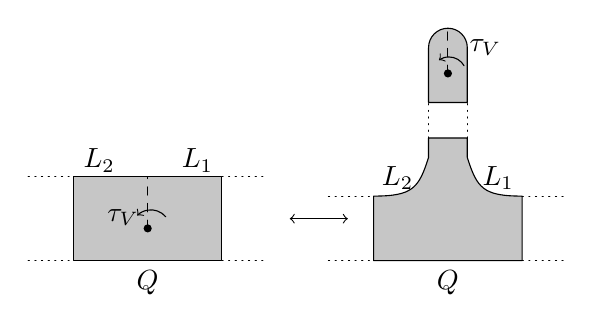
\begin{tikzpicture}[line cap=round,line join=round,scale=0.82]
\draw[dotted] (-0.7,1.3) -- (0,1.3);
\draw[dotted] (-0.7,0) -- (0,0);
\draw[fill=gray!45] (0,0) rectangle (2.3,1.3);
\fill (1.15,0.5) circle (1.8pt);
\draw[dashed] (1.15,0.5) -- (1.15,1.3);
\draw[->] (1.43,0.68) arc[start angle=40,end angle=135,radius=0.3];
\node at (0.77,0.67) {$\tau_V$};
\node at (0.4,1.55) {$L_2$};
\node at (1.92,1.55) {$L_1$};
\node at (1.15,-0.34) {$Q$};
\draw[dotted] (2.3,1.3) -- (2.95,1.3);
\draw[dotted] (2.3,0) -- (2.95,0);
\draw[<->] (3.35,0.65) -- (4.25,0.65);
\draw[dotted] (3.95,1.0) -- (4.65,1.0);
\draw[dotted] (3.95,0) -- (4.65,0);
\draw[fill=gray!45]
  (4.65,0) -- (4.65,1.0)
  .. controls (5.25,1.0) and (5.35,1.12) .. (5.5,1.6)
  -- (5.5,1.9) -- (6.1,1.9) -- (6.1,1.6)
  .. controls (6.25,1.12) and (6.35,1.0) .. (6.95,1.0)
  -- (6.95,0) -- cycle;
\node at (5.02,1.28) {$L_2$};
\node at (6.58,1.28) {$L_1$};
\node at (5.8,-0.34) {$Q$};
\draw[dotted] (5.5,1.9) -- (5.5,2.45);
\draw[dotted] (6.1,1.9) -- (6.1,2.45);
\draw[fill=gray!45] (5.5,2.45) -- (5.5,3.3) arc[start angle=180,end angle=0,radius=0.3] -- (6.1,2.45) -- cycle;
\fill (5.8,2.9) circle (1.8pt);
\draw[dashed] (5.8,2.9) -- (5.8,3.55);
\draw[->] (6.05,3.02) arc[start angle=30,end angle=125,radius=0.27];
\node at (6.38,3.3) {$\tau_V$};
\draw[dotted] (6.95,1.0) -- (7.6,1.0);
\draw[dotted] (6.95,0) -- (7.6,0);
\end{tikzpicture}
\caption{}\label{fig:xi-family}
\end{figure}
$\psi$ 的定义始于写下五个由\trLefschetzFibration{}组成的单参数\trFamily，每个都配备有\trBoundaryCondition{}与\trPerturbationDatum，它们共同组成一条闭的链（前一个的终点是后一个的起点，依此类推；图形化的展示见\cref{fig:psi-chain}）。第一个\trFamily{}就是上面定义的 $E^{l,r}\to S^{l,r}$。为得到第二个（将记作 $E^{\xi(\mu^2),r}\to S^{\xi(\mu^2),r}$），我们取 $E^{\xi,r}\to S^{\xi,r}$，把它的唯一的出向端\trGluing{}到三\trPointedDisc{}上一个平凡\trFibration{}的入向端上；后面这一块带有\trBoundaryCondition{}$Q$、$L_0$、$L_1$，以及定义 $\mu^2$ 乘积的那个\trPerturbationDatum。于是，只要\trGluingLength{}取得足够大，对这个由\trFibration{}组成的\trFamily{}的\trPseudoholomorphic\trSection{}作计数就恰好给出 $\xi(\mu^2(\cdot,\cdot))$。回忆一下，$E^{l,1}\to S^{l,1}$ 是通过取 $E^d\to S^d$ 再粘入三\trPointedDisc{}上的一个平凡\trFibration{}而得到的；另一方面，按定义我们有 $(E^{\xi,0}\to S^{\xi,0})=(E^d\to S^d)$。这意味着：只要把\trGluingParameter{}取得合适，就有
\begin{equation}\label{eq:xi-mu2-endpoint}
\bigl(E^{\xi(\mu^2),0}\to S^{\xi(\mu^2),0}\bigr)=\bigl(E^{l,1}\to S^{l,1}\bigr),
\end{equation}
这里的相等也包括\trBoundaryCondition{}与\trPerturbationDatum。在另一端，即 $r=1$ 处，我们有一个\trFibration{}$E^{\xi(\mu^2),1}\to S^{\xi(\mu^2),1}$，它给出表达式 $\mu^2(c,\mu^2(\cdot,\cdot))$。这立刻暗示了下一步的做法：取一个充分大的闭区间 $[0;1]\subset\scr{R}^4$，考虑其上四\trPointedDisc{}的\trUniversal\trFamily，各\trBoundaryComponent{}由 $(Q,L_0,L_1,L_2)$ 来标记。把它变成一个由平凡\trLefschetzFibration{}组成的\trFamily，配以各自恰当的\trBoundaryCondition{}与\trPerturbationDatum，然后把每个\trDisk{}的第三个出向端\trGluing{}到 $E^c\to S^c$ 的入向端上。我们把所得结果记作 $E^{\mu^3(c\otimes\mathrm{Id}),r}\to S^{\mu^3(c\otimes\mathrm{Id}),r}$，因为对这个\trFamily{}中的\trPseudoholomorphic\trSection{}作计数恰好产生 $\mu^3(c,\cdot,\cdot)$。通过对\trGluingParameter{}的适当选取，必定能够做到
\begin{equation*}
\bigl(E^{\mu^3(c\otimes\mathrm{Id}),0}\to S^{\mu^3(c\otimes\mathrm{Id}),0}\bigr)=\bigl(E^{\xi(\mu^2),1}\to S^{\xi(\mu^2),1}\bigr)
\end{equation*}
其意义与 \eqref{eq:xi-mu2-endpoint} 中的相同。在另一个极端 $r=1$ 处，我们得到一个\trLefschetzFibration，它的\trSection{}定义出\trHomomorphism{}$\mu^2(\mu^2(c,\cdot),\cdot)$。对第四个\trFamily{}$E^{\mu^2(k\otimes\mathrm{Id}),r}\to S^{\mu^2(k\otimes\mathrm{Id}),r}$，我们取\trBoundaryComponent{}由 $(Q,L_0,L_2)$ 来标记的三\trPointedDisc，把它变成一个平凡\trLefschetzFibration，然后把它的第二个出向端与诸\trFibration{}$E^{k,r}\to S^{k,r}$ 的入向端\trGluing{}起来。由 $k$ 的定义，
\begin{equation*}
\bigl(E^{\mu^2(k\otimes\mathrm{Id}),0}\to S^{\mu^2(k\otimes\mathrm{Id}),0}\bigr)=\bigl(E^{\mu^3(c\otimes\mathrm{Id}),1}\to S^{\mu^3(c\otimes\mathrm{Id}),1}\bigr).
\end{equation*}
\begin{figure}[p]
\centering
\begin{tikzpicture}[line cap=round,line join=round,scale=0.62]
\draw[fill=gray!45,rounded corners=9pt]
  (0,1.48) -- (0,2.35)
  .. controls (0.8,2.35) and (1.3,2.7) .. (2.1,3.35)
  -- (2.5,3.0)
  .. controls (1.95,2.4) and (1.8,2.3) .. (1.7,2.12)
  .. controls (1.8,1.95) and (2.05,1.65) .. (2.4,1.3)
  -- (2.06,0.94)
  .. controls (1.6,1.3) and (1.1,1.5) .. (0,1.48) -- cycle;
\draw[dotted] (2.28,2.5) .. controls (2.6,2.4) .. (2.78,2.25);
\draw[dotted] (2.24,1.62) .. controls (2.55,1.68) .. (2.78,1.78);
\draw[fill=gray!45] (3.32,2.0) circle (0.55);
\fill (3.32,2.0) circle (1.8pt);
\node at (1.05,3.85) {$0$（消没）};
\draw[<->] (4.15,2.0) -- (5.25,2.0);
\node at (4.7,2.3) {$l$};
\draw[fill=gray!45] (5.5,1.7) rectangle (6.9,2.3);
\fill (6.2,2.0) circle (1.8pt);
\node at (6.2,2.62) {$d(\mu^2)$};
\draw[dotted] (6.9,2.25) -- (7.5,2.25);
\draw[dotted] (6.9,1.75) -- (7.5,1.75);
\draw[fill=gray!45]
  (7.5,2.25)
  .. controls (8.1,2.35) and (8.5,2.6) .. (8.85,2.85)
  -- (8.85,2.3) arc[start angle=90,end angle=270,radius=0.3]
  .. controls (8.4,1.5) and (8.0,1.68) .. (7.5,1.75) -- cycle;
\draw[<->] (8.2,1.15) -- (8.2,0.25);
\node at (9.15,0.7) {$\xi(\mu^2)$};
\draw[fill=gray!45] (6.55,0.05) circle (0.5);
\fill (6.55,0.05) circle (1.8pt);
\draw[dotted] (6.3,-0.45) -- (6.3,-0.9);
\draw[dotted] (6.8,-0.45) -- (6.8,-0.9);
\draw[fill=gray!45]
  (5.45,-1.4) -- (6.05,-1.4)
  .. controls (6.28,-1.4) and (6.3,-1.15) .. (6.3,-0.9)
  -- (6.8,-0.9)
  .. controls (6.8,-1.15) and (6.82,-1.4) .. (7.05,-1.4)
  -- (7.55,-1.4) -- (7.55,-2.15) -- (5.45,-2.15) -- cycle;
\draw[dotted] (7.55,-1.95) -- (8.15,-1.95);
\draw[dotted] (7.55,-1.6) -- (8.15,-1.6);
\draw[fill=gray!45]
  (8.15,-1.6)
  .. controls (8.7,-1.5) and (9.05,-1.3) .. (9.4,-1.05)
  -- (9.4,-1.6) arc[start angle=90,end angle=270,radius=0.28]
  .. controls (9.0,-2.05) and (8.6,-2.1) .. (8.15,-1.95) -- cycle;
\node at (9.45,-0.5) {$\mu^2(c,\mu^2)$};
\draw[<->] (8.35,-2.4) -- (8.35,-3.3);
\node at (9.5,-2.85) {$\mu^3(c\otimes\mathrm{Id})$};
\draw[fill=gray!45] (7.5,-3.85) circle (0.5);
\fill (7.5,-3.85) circle (1.8pt);
\draw[dotted] (7.25,-4.35) -- (7.25,-4.8);
\draw[dotted] (7.75,-4.35) -- (7.75,-4.8);
\draw[fill=gray!45]
  (7.15,-4.8) -- (7.15,-6.0) -- (7.85,-6.0)
  -- (7.85,-5.7) arc[start angle=-90,end angle=90,radius=0.3] -- (7.85,-4.8) -- cycle;
\draw[dotted] (7.25,-6.0) -- (7.25,-6.45);
\draw[dotted] (7.75,-6.0) -- (7.75,-6.45);
\draw[fill=gray!45]
  (7.2,-6.45)
  .. controls (6.9,-6.5) and (6.6,-6.8) .. (6.5,-7.15)
  -- (8.5,-7.15)
  .. controls (8.4,-6.8) and (8.1,-6.5) .. (7.8,-6.45) -- cycle;
\node at (7.6,-7.72) {$\mu^2(\mu^2(c\otimes\mathrm{Id})\otimes\mathrm{Id})$};
\draw[<->] (1.6,0.7) -- (1.6,-4.95);
\node at (2.6,-2.1) {$0$（消没）};
\draw[fill=gray!45] (1.25,-2.3) rectangle (1.95,-3.5);
\draw[dotted] (1.95,-2.7) -- (2.5,-2.7);
\draw[dotted] (1.95,-3.1) -- (2.5,-3.1);
\draw[fill=gray!45] (2.85,-2.9) circle (0.5);
\fill (2.85,-2.9) circle (1.8pt);
\draw[dotted] (1.4,-3.5) -- (1.4,-3.95);
\draw[dotted] (1.8,-3.5) -- (1.8,-3.95);
\draw[fill=gray!45]
  (1.3,-4.6)
  .. controls (1.0,-4.62) and (0.6,-4.9) .. (0.5,-5.3)
  -- (2.75,-5.3)
  .. controls (2.65,-4.9) and (2.25,-4.62) .. (1.9,-4.6) -- cycle;
\node at (1.65,-5.9) {$\mu^2(0\otimes\mathrm{Id})$（消没）};
\draw[<->] (3.7,-4.35) -- (6.3,-4.35);
\node at (5.0,-3.92) {$\mu^2(k\otimes\mathrm{Id})$};
\end{tikzpicture}
\caption{}\label{fig:psi-chain}
\end{figure}
另一方面，对 $r=1$，我们可以把 $E^{\mu^2(k\otimes\mathrm{Id}),1}$ 设想成是按如下方式构造出来的：从一个三\trPointedDisc{}上的平凡\trFibration{}出发，其\trBoundaryCondition{}在两条\trBoundaryComponent{}上是常值的且分别等于 $Q$ 与 $L_0$，而在剩下那一条上实现从 $\tau_V(L_1)$ 到 $L_2$ 的\trIsotopy。在 $L_0$ 那条分支上标记一个边界点，并如 $k$ 的定义中那样，与 $E$（带着它的标准\trBoundaryCondition）作\trBoundaryConnectedSum。注意，$E^{l,0}\to S^{l,0}$ 当初就是以本质上相同的方式定义的。细节（比如那个\trMarkedPoint{}的位置）可能有所不同，但显然可以用第五个也是最后一个\trFamily{}（记作 $E^{0,r}\to S^{0,r}$）在二者之间进行过渡；这个\trFamily{}具有如下性质：每个 $E^{0,r}$ 都是通过与 $E$ 作\trBoundaryConnectedSum{}而得到的，其中\trGluingParameter{}\emph{始终保持很小}。按定义，这就完成了我们的链：
\begin{equation*}
\begin{gathered}
\bigl(E^{0,0}\to S^{0,0}\bigr)=\bigl(E^{\mu^2(k\otimes\mathrm{Id}),1}\to S^{\mu^2(k\otimes\mathrm{Id}),1}\bigr),\\
\bigl(E^{0,1}\to S^{0,1}\bigr)=\bigl(E^{l,0}\to S^{l,0}\bigr).
\end{gathered}
\end{equation*}
\cref{thm:cochain-level-vanishing} 中的诸消没结果将以适当\trParametrization{}的版本适用于 $E^{0,r}\to S^{0,r}$，因此与之相关联的那些由\trPseudoholomorphic\trSection{}组成的零维\trModuliSpace{}的计数将是平凡的。最后，整条链构成一个以 $S^1$ 为参数的、由\trLefschetzFibration{}组成的\trFamily，它显然可以用一个定义在 $D^2$ 上的\trFamily{}来\trFilling。我们用由此得到的\trParametrization{}\trModuliSpace{}来定义 $\psi$，于是 \eqref{eq:xi-psi} 将由构造成立。
\begin{remark}\label{thm:standardized-framework}
把这个过程纳入一个更一般且更标准化的框架中来考察是很有启发性的。令 $\scr{R}^{3,1}$ 是带一个额外内部\trMarkedPoint{}的三\trPointedDisc{}的\trModuliSpace。\trEquivalence{}地——这对我们的目的而言也更合适——可以固定内部点与第一个边界点（这就打破了 $\mathrm{Aut}(D)$ 对称性），而把 $\scr{R}^{3,1}$ 看成其余两个边界点的\trConfigurationSpace。取\trDisk{}$D$ 作为我们的标准\trLefschetzFibration{}$E\to S$ 的基，其内部\trMarkedPoint{}为唯一的\trCriticalValue，而第一个边界点为 $\ast$。对任何构型 $(z_1,z_2)\in\scr{R}^{3,1}$，我们可以把 $E$ 限制到 $S\setminus\{\ast,z_1,z_2\}$ 上，并把这个限制变成一个带\trStriplikeEnd{}的\trLefschetzFibration。给这个由\trFibration{}组成的\trFamily{}配备由 $Q$、$L_0$、$L_1$ 以及从 $\tau_V(L_1)$ 到 $L_2$ 的\trIsotopy{}组成的\trLagrange\trBoundaryCondition；并考察由此得到的\trParametrization{}\trModuliSpace{}给出的\trInvariant。
为了理解它所满足的关系，我们需要考察 \trDeligne--\trMumford{}式的\trCompactification{}$\overline{\scr{R}}^{3,1}$，它是一个六边形（正如 $\overline{\scr{R}}^5$ 一样，它可以实现为复 \trDeligne--\trMumford{}空间 $\overline{\scr{M}}_{0,5}$ 的\trRealLocus，所对应的\trAntiholomorphic\trInvolution{}把复共轭与两个\trMarkedPoint{}的对换结合在了一起）。与各条\trStratum{}相对应的\trDegenerate{}情形示于\cref{fig:hexagon-degenerations}。对于边 (i) 与 (ii)，相应的单参数\trFamily{}是\cref{fig:psi-chain} 中那些\trFamily{}的极限（让\trGluingParameter{}趋于零），给出 \eqref{eq:xi-psi} 中的项 $\mu^3(c\otimes\mathrm{Id})$ 与 $\mu^2(k\otimes\mathrm{Id})$。图中的其余部分稍更复杂一些：产生我们的 $\xi(\mu^2)$ 项的那个\trFamily{}对应于边 (vi) 的一部分，而 $E^{0,r}\to S^{0,r}$ 类似地盖住边 (iii) 的一部分；这两条边的其余部分，以及 (iv) 与 (v)，在\cref{fig:psi-chain} 中没有直接的对应物，但它们的并可以相对于端点作\trDeformation，变成产生 $l$ 的那个单参数\trFamily。所以，从图形上讲，\cref{fig:psi-chain} 中的五个\trFamily{}可以被看成 \cref{fig:hexagon-degenerations} 中的那些虚线边。就实际目的而言，这意味着：如果直接使用 $\overline{\scr{R}}^{3,1}$ 本身，那么所得结果将是 \eqref{eq:auxiliary-complex-maps} 与 \eqref{eq:xi-psi} 的稍更复杂的版本（含更多的项）。
\end{remark}
\begin{figure}[p]
\centering
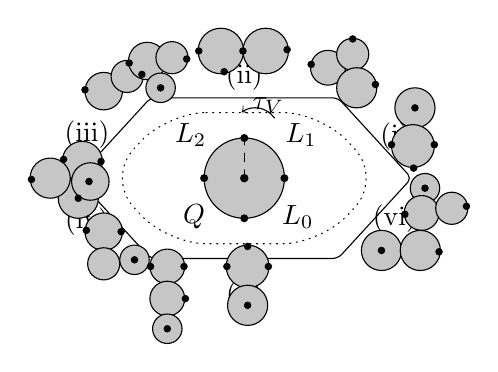
\begin{tikzpicture}[line cap=round,line join=round,scale=0.85]
\draw[rounded corners=2pt]
  (-0.2,1.2) -- (0.9,2.4) -- (3.7,2.4) -- (4.8,1.2) -- (3.7,0.0) -- (0.9,0.0) -- cycle;
\draw[dotted,rounded corners=14pt]
  (1.15,2.18) -- (3.45,2.18) -- (4.35,1.2) -- (3.45,0.22) -- (1.15,0.22) -- (0.25,1.2) -- cycle;
\draw[fill=gray!45] (2.3,1.2) circle (0.6);
\fill (2.3,1.2) circle (1.8pt);
\fill (1.7,1.2) circle (1.7pt);
\fill (2.9,1.2) circle (1.7pt);
\fill (2.3,0.6) circle (1.7pt);
\fill (2.3,1.8) circle (1.7pt);
\draw[dashed] (2.3,1.2) -- (2.3,1.8);
\draw[->] (2.75,2.1) arc[start angle=35,end angle=125,radius=0.35];
\node at (2.66,2.28) {$\tau_V$};
\node at (1.5,1.85) {$L_2$};
\node at (3.15,1.85) {$L_1$};
\node at (1.55,0.62) {$Q$};
\node at (3.1,0.62) {$L_0$};
\node at (2.3,2.72) {(ii)};
\node at (4.55,1.82) {(i)};
\node at (4.55,0.6) {(vi)};
\node at (2.3,-0.55) {(v)};
\node at (-0.05,0.55) {(iv)};
\node at (-0.05,1.85) {(iii)};
\foreach \x/\y/\r in {
    0.2/2.5/0.28, 0.55/2.72/0.24,
    0.85/2.95/0.28, 1.22/3.0/0.24, 1.05/2.55/0.22,
    1.95/3.1/0.34, 2.62/3.1/0.34,
    3.55/2.85/0.26, 3.92/3.05/0.24, 3.98/2.55/0.3,
    4.85/2.25/0.3, 4.82/1.68/0.32,
    5.0/1.05/0.22, 4.95/0.68/0.26, 5.4/0.75/0.24,
    4.35/0.12/0.3, 4.93/0.12/0.3,
    2.35/-0.12/0.32, 2.35/-0.7/0.3,
    1.15/-0.12/0.26, 1.15/-0.6/0.26, 1.15/-1.05/0.22,
    0.2/0.4/0.28, 0.2/-0.08/0.24, 0.66/-0.02/0.22,
    -0.12/1.45/0.3, -0.18/0.9/0.3,
    -0.6/1.2/0.3, 0.0/1.15/0.28}
  {\draw[fill=gray!45] (\x,\y) circle (\r);}
\foreach \x/\y in {
    -0.08/2.52, 0.77/2.75,
    0.58/2.92, 1.44/2.98, 1.05/2.55,
    1.62/3.1, 2.28/3.1, 2.94/3.12, 2.0/2.79,
    3.3/2.9, 3.92/3.28, 4.26/2.6,
    4.85/2.25, 4.5/1.7, 5.14/1.7, 4.83/1.35,
    5.0/1.05, 4.7/0.66, 5.62/0.78,
    4.35/0.12, 5.21/0.1,
    2.35/0.18, 2.04/-0.12, 2.66/-0.12, 2.35/-0.7,
    0.9/-0.12, 1.4/-0.12, 1.42/-0.6, 1.15/-1.05,
    -0.06/0.42, 0.46/0.4, 0.66/-0.02,
    -0.4/1.48, 0.16/1.45, -0.18/0.9,
    -0.88/1.18, -0.02/1.15}
  {\fill (\x,\y) circle (1.6pt);}
\end{tikzpicture}
\caption{}\label{fig:hexagon-degenerations}
\end{figure}
\begin{remark}\label{thm:c1-correction-chains}
在我们后面的应用中，条件 $2c_1(M,V)=0$ 将总是成立的，这是\trGrading{}存在性的一个推论（见 \cref{sub:lagrangian-branes} 中的讨论）。尽管如此，如有必要，也可以通过添加涉及适当限制链的修正项来省去这个条件，一如 [131, Lemma 3.12] 或上文的 \cref{thm:fibre-product-vanishing}。
\end{remark}
